\section{Smooth Manifolds}

\begin{definition}
    We call a map $f:\R^n \xrightarrow{} \R^n$ \textbf{$q$-smooth}, or $C^q$, if
    it has continuous partial derivatives of order  $q$. We call  $f$
    \textbf{smooth}, or $C^\infty$, if it has continuous partial derivatives of
    all orders.
\end{definition}

\begin{definition}
    A \textbf{$C$-smooth manifold}, or  \textbf{$C^q$-manifold} with $q>0$ is a
    topological manifold with an atlas that is  $C^q$. That is, for any charts
    $(M_\a,\phi_\a)$ and $(M_\b,\phi_\b)$, $\phi_\b \circ \inv{\phi_\a}$ is $C^q$
    wherever it is defined. We call  $C^\infty$-manifolds  \textbf{smooth manifolds},
    or \textbf{differentiable manifolds}. We call the maps $\phi_\b \circ
    \inv{\phi_\a}$ \textbf{transition maps}.
\end{definition}

\begin{example}\label{example_1.6}
    \begin{enumerate}
        \item[(1)] $\R^n$ is a smooth manifold, as are all its open subsets.

        \item[(2)] Consider the $n$-manifold  $S^n$ with charts
            \begin{align*}
                (\com{S^n}{(0, \dots, 0,1)},h) && (\com{S^n}{(0, \dots, 0,-1)},h')  \\
            \end{align*}
            where
            \begin{equation*}
                h(x_1, \dots,x_{n+1})=\frac{1}{1-x_{n+1}}(x_1, \dots x_n) \text{
                and } h'(x_1, \dots,x_{n+1})=\frac{1}{1+x_{n+1}}(x_1, \dots x_n)
            \end{equation*}
            The map $h' \circ \inv{h}$ is smooth. Notice that
            \begin{equation*}
                \inv{h}(y_1, \dots,y_n)=\Big{(}\frac{2y_1}{1+y_1^2+\dots+y_n^2},
                \dots, \frac{2y_n}{1+y_1^2+\dots+y_n^2}\Big{)}
            \end{equation*}
            So that
            \begin{equation*}
                h' \circ \inv{h}=\frac{1}{y_1^2+\dots+y_n^2}(y_1, \dots, y_n)
            \end{equation*}
            Moreover, for all $q>0$, $\partial^q{h' \circ \inv{h}}$ exists,
            which makes $h' \circ \inv{h}$ smooth. This makes $S^n$ a smooth
            manifold.

        \item[(3)] The product of smooth manifolds are smooth manifolds. In
            particular, the torus $T^2=S^1 \times S^1$ is a smooth manifold.
    \end{enumerate}
\end{example}

\begin{definition}
    Let $M$ and $N$ manifolds with atlases  $\{(M_\a,\phi_\a)\}$ and $\{(N_\b,
    \psi_\b)\}$. We call a map $f:M \xrightarrow{} N$ \textbf{$q$-smooth}, or
    $C^q$ if  $\psi_\b \circ \inv{\phi_\a}$ is $C^q$ wherever it is defined. We
    call  $C^q$-maps between manifolds  \textbf{$C^q$-diffeomorphisms}. We call
    $C^\infty$-diffeomorphisms  \textbf{diffeomorphisms}. We call any two
    $C^q$-manifolds  \textbf{diffeomorphic} if there exists a
    $C^q$-diffeomorphism between them.
\end{definition}

\begin{example}\label{example_1.7}
    \begin{enumerate}
        \item[(1)] The map $f:\R \xrightarrow{} \R$ given by $f(x)=x^3$ is a
            smooth map, but it is not a diffeomorphism, since $f'(x)=3x^2$ has a
            singular point at $0$ (elaborate?). It is not even a
            $C^1$-diffeomorphism.

        \item[(2)] The projection map of $T^2=S^1 \times S^1$ onto the second
            factor is a smooth map between manifolds.
    \end{enumerate}
\end{example}

\begin{definition}
    Let $M$ a  $C^q$-manifold, for some  $q \geq 1$, and let  $x \in M$ and
    $(M_\a,\phi_\a)$ a chart containing $x$. We call  $x$ a  \textbf{critical
    point} of a map $f:M \xrightarrow{} \R$ if it is a critical point of  $f \circ
    \inv{\phi_\a}$. If $g:\R^n \xrightarrow{} \R^n$ is a map, we call $x$ a
     \textbf{nondegenerate} critical point if the Hessian of $g$ is nonsingular
     at  $x$, and we call  $x$ a  \textbf{nondegenerate} critical point of $f$
     if it is a nondegenerate critical point of $f \circ \inv{\phi_\a}$.
\end{definition}

\begin{definition}
    We define a \textbf{Morse function} on a manifold $M$ to be a smooth map
    $f:M \xrightarrow{} \R$ such that
    \begin{enumerate}
        \item[(1)] $f$ has nondegenerate critical points.

        \item[(2)] Distinct critical points map to distinct values.
    \end{enumerate}
\end{definition}

\begin{example}\label{1.8}
    The projection map of the Torus $T^2 \subseteq \R^3$ on to the third
    coordinate is a map with critical points. It has $1$ maximum value,  $2$
    minimum values, and  $2$ saddle points. Moreover these critical points are
    nondegenerate, so that the projection is a Morse function. Notice that these
    critical points are nondegenerate, since they consist of minima, maxima, and
    saddle points. Moreover, we see that the sum of the minima and maxima, minus
    the saddle points is $1+1-2=0$.
    \begin{figure}[h]
        \centering
        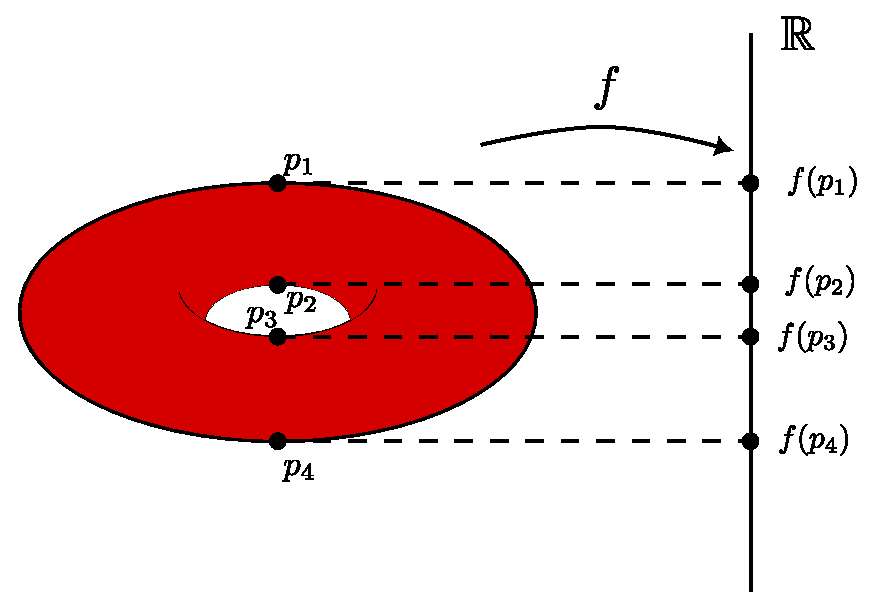
\includegraphics[scale=0.5]{Figures/chapter1/morse_func_torus.eps}
        \caption{A Morse function on the torus $T^2$.}
        \label{figure_1.5}
    \end{figure}
\end{example}

\begin{definition}
    A \textbf{$q$-smooth submanifold}, or  \textbf{$C^q$-submanifold} of a
     $C^q$-manifold  $M$ is a  $p$-dimensional submanifold of $M$ for which the
     transition maps restricted to $L$ are  $C^q$.
\end{definition}

\begin{definition}
    A  \textbf{$q$-smooth manifold}, or \textbf{$C^q$-manifold} with
    \textbf{boundary} $M$ is a topological manifold with boundary such that for any
    charts $(M_\a,\phi_\a)$ and $(M_\b,\phi_\b)$ in the atlas of $M$, the
    transition map  $\phi_\b \circ \inv{\phi_\a}$ is $C^q$ wherever it is
    defined. We call $C^\infty$ manifolds with boundary  \textbf{smooth
    manifolds}, or \textbf{differentiable manifolds} with \textbf{boundary}.
\end{definition}
